\section{Learning Pong}

After papers like "Reward is enough"\cite{silver2021reward} and "Playing Atari with Deep Reinforcement Learning"\cite{mnih2013playing} the enthusiasm for the RL has risen more and more.
"Reward is enough" hypothesizes how intelligence can be understood as subservient to reward maximization. The reward is enough to drive behavior that displays skills studied in natural and artificial intelligence. This is in contrast to the idea that specialized problem formulations, based on other signals or goals, are required for each skill \cite{silver2021reward}.

"Imitative Policies for Reinforcement Learning" \cite{dahlstrom2002imitative} describes a way to apply the Q-learning algorithm to the game of Pong. Moreover, it wants to use the moves made by experts as observations in order to speed up the learning process. 
The pong board is a 10x12 rectangle and the agent controls a paddle of width 2, which can move one position to the right or left.
An integral horizontal velocity ranging from -2 to +2 units is added every time step. Hitting the ball yields a +1 reward; missing it yields a -1 penalty.

"Playing Atari with Deep Reinforcement Learning" presents the first deep learning model to successfully learn control policies directly from high-dimensional sensory inputs (raw pixels) using Reinforcement Learning \cite{mnih2013playing}.

In this work seven popular ATARI games were considered including pong.

Game frames was captured at a resolution of 210x160 gray-scale, down-sampling it to a 110x84 image, cropped to a 84x84 patch of the playing area
and given in input to a modified version of a CNN for RL (Deep Q Network).

A frame skipping technique is used to play roughly k times more games without significantly increasing the runtime.

The network has an input shape of 84x84x4 and has a separate output unit for each possible action, the number of which depends on the games considered (between 4 and 18 in this case).
For all the games considered all positive rewards are fixed to be 1 and all negative rewards to be -1.

A variant of online Q-Learning that combines stochastic mini-batch updates with experience replay memory was used to ease the training of deep RL networks.
The network was trained with an $\epsilon$-greedy annealed strategy for a total of 10 million frames and a replay memory of one million most recent frames was used.




Another work that use DQN is "Learning to Play Pong Video Game via Deep Reinforcement Learning" where they focus on pong only.
The reward considered is the same as in "Playing Atari with Deep Reinforcement Learning" +1 when the agent score a point -1 when the opponent score a point.
The screenshots with a fixed 32 FPS are binarized and rescaled to 80x80.
Agent actions considered are move paddle up, move paddle down, paddle stays at the same place.
In particular they added an Episodic Control technique, implemented with an embedding function represented as a random projection, to reuse successful strategies.




The "Learning to Coordinate with Deep Reinforcement Learning in Doubles Pong Game" discusses the emergence of cooperative and coordinated behaviors between joint and concurrent learning
agents using deep Q-learning, by considering a scenario where 2 agents DQN`s form a team to win against an hard-coded AI,
and automatically learn how to cooperate and divide the space of their side of the field.

\begin{figure}[ht]
  \centering
  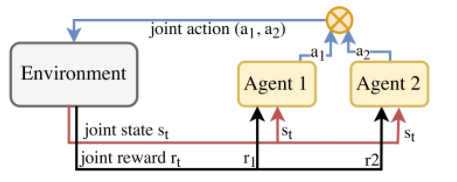
\includegraphics[width=0.4\textwidth]{images/DQN_MAS.png}
  \label{dqnmas}
  \caption{DQN adapted to MAS.}
\end{figure}

There are three actions that each agent can take: move up, move down, stay at the same place.

\begin{table}[ht]
  \centering
  \begin{tabular}{@{}ccc@{}}
    \toprule
    \textbf{Events}            & \textbf{Agent 1 reward} & \textbf{Agent 2 reward} \\ \midrule
    \textbf{Left player loses} & +1                      & +1                      \\
    \textbf{One agent loses}   & -1                      & -1                      \\
    \textbf{Collision}         & -1                      & -1                      \\ \bottomrule
  \end{tabular}
  \label{my-table}
  \caption{reward scheme adopted.}
\end{table}

Instead of randomly sampling prioritized experience replay is used.




All previous works make the agent learn to play pong against an hardcoded AI agent, but "Multi agent cooperation and competition with deep reinforcement learning" considered to use an opponent
which is Learning too and showed that this can further improve the robustness of the model when playing with others different opponent.

Multiple agents controlled by autonomous DQNs learn to cooperate and compete while sharing a high-dimensional environment and being fed only raw visual input
There are 4 actions that each of the two agents can take: move up, move down, stand still, and fire (to relaunch the ball or to start the game).

\noindent
3 rewarding scheme:
\begin{itemize}
  \item Score more than the opponent (fully competitive) $\rightarrow \rho = 1$.
  \item Loosing the ball penalizes both players (fully cooperative) $\rightarrow \rho = $ -1.
  \item Transition between cooperation and competition $\rightarrow \rho = range(-1, 1, 0.25)$.
\end{itemize}

\begin{table}[ht]
  \centering
  \begin{tabular}{c|c|c|}
    \cline{2-3}
                                                   & \textbf{L player scores} & \textbf{R player scores} \\ \hline
    \multicolumn{1}{|c|}{\textbf{L player scores}} & $\rho$                   & -1                       \\ \hline
    \multicolumn{1}{|c|}{\textbf{R player scores}} & -1                       & $\rho$                   \\ \hline
  \end{tabular}
  \caption{general rewarding scheme.}
  \label{tab:my-table2}
\end{table}


A different is "LEARNING PONG" which uses a neural network automatically generated with genetic algorithms to let the agents learn to play Pong, in this case no scripted opponent AI.

A Custom version of Pong is considered where the goals are smaller and the players have the ability to move in both the x and y dimensions.

The state is represented as eight inputs: the paddle's X and Y position, the opponent's X and Y position, the ball's X and Y velocity,
and the ball's X and Y position and the output of the neural network has four output nodes: to movement up, down, left and right.

Two algorithms were used the NeuroEvolution(NE) and NeuroEvolution of Augmenting Topologies(NEAT).
The first start from a predefined neural net structure and iteratively tune its parameters, while the second adds the possibility to modify the network topology by adding nodes and connections randomly.



\begin{figure}[ht]
  \centering
  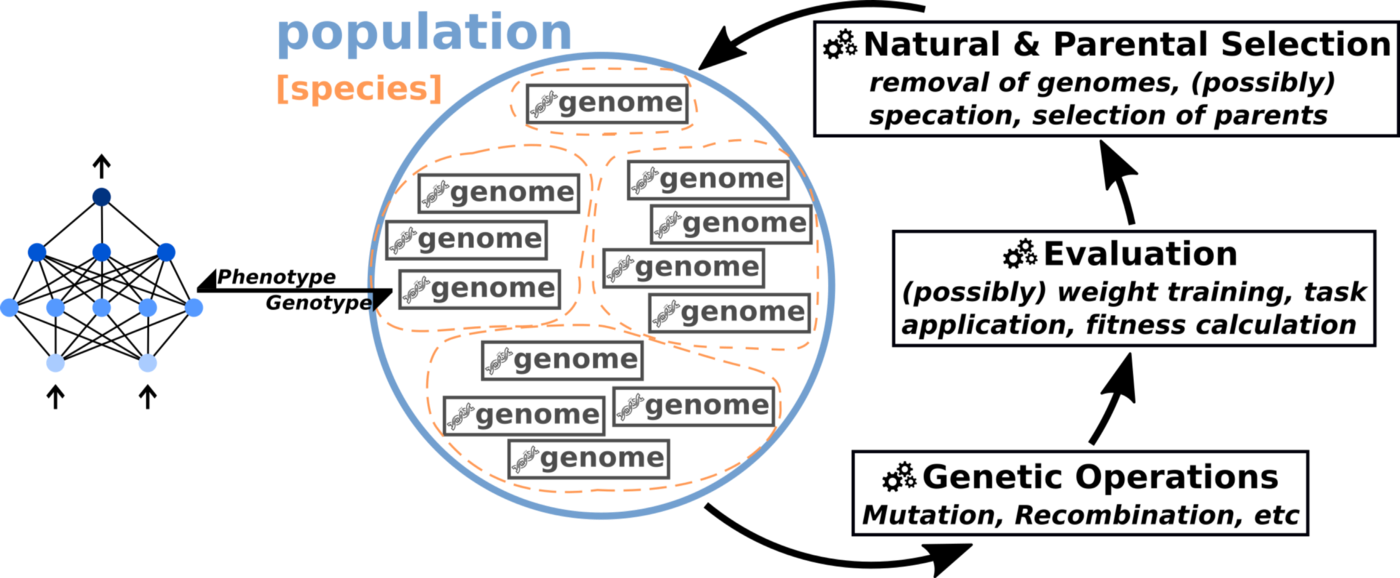
\includegraphics[width=0.4\textwidth]{images/neuroevolution.png}
  \label{ne}
  \caption{NeuroEvolution algorithm schema.}
\end{figure}
